\chapter{\label{ch:7-qbo} QBO Teleconnections in the UM with a nudged stratosphere }

The previous chapter describes QBO teleconnections in the MOHC CMIP6 pre-industrial control experiments. One could reasonably hypothesize that those relationships are the result of a control of tropical convection by the QBO. 
This chapter tests this hypothesis by constraining the zonal winds in the tropical stratosphere, eliminating any possible influence of the troposphere on the stratosphere. 
The relaxation experiment design is described and results are presented and a discussion on how the nudging modifies the teleconnections found in the free-running CMIP6 experiments is given at the end of the chapter. 

\section{Introduction}

The use of GCMs to address these questions is also limited due to the fact that only some recent models are able to reproduce a sufficiently reasonable representation of the QBO, and even so, some of the models in the CMIP6 produce highly unrealistic QBO features \citep{richter2020}. 
Some of these biases have led several studies to perform experiments in which a GCM is relaxed towards an observed or idealized state where the model is forced to reproduce a sensible QBO signal \citep{gray2020,richter2020,martin2021}. 

This chapter first makes a case for nudging experiment, described the experimental configuration and the goals and hypotheses that we aim to test using these simulations. 
% analysis of the pre-industrial control simulations is followed by a short section that makes the case for the use of nudging experiments using the UM to further investigate the findings of the first section. 
Then, a description of the experimental setup is given and finally, results comparing runs using the nudging technique versus the free running model are presented and discussed highlighting the possible mechanisms at play for the tropical route of QBO teleconnections. 

\section{The case for nudging}

Global climate models exhibit a number of biases in their representation of various aspects of the climate, all of which lead to uncertainty in our ability to make statements about the real-world based on their results. One example of a key bias discussed in this thesis is the magnitude and position of precipitation associated with the ITCZ in the Atlantic Ocean, which is associated with biases in South American precipitation. % the mean state of the Pacific and Atlantic SSTs as well as many others. 
For this section, one relevant bias to consider is how current models represent the tropical stratosphere and, in particular, their representation of the QBO.

The number of GCMs with a full stratosphere have increased notably from CMIP3 to CMIP6 which means that features such as the QBO are increasingly better resolved with each iteration of the CMIP \citep{bushell2020,richter2020}. Nevertheless, several aspects of the QBO are still not well represented by state-of-the-art climate models, such as the period and amplitude of the QBO \citep{schenzinger2017,richter2020}. 
These biases increase uncertainty in teleconnections diagnosed from these models, because these biases could make the models misrepresent processes that are observed in the real-world between the tropical stratosphere and troposphere.

\begin{figure}[t!]
\centering
 %\noindent
 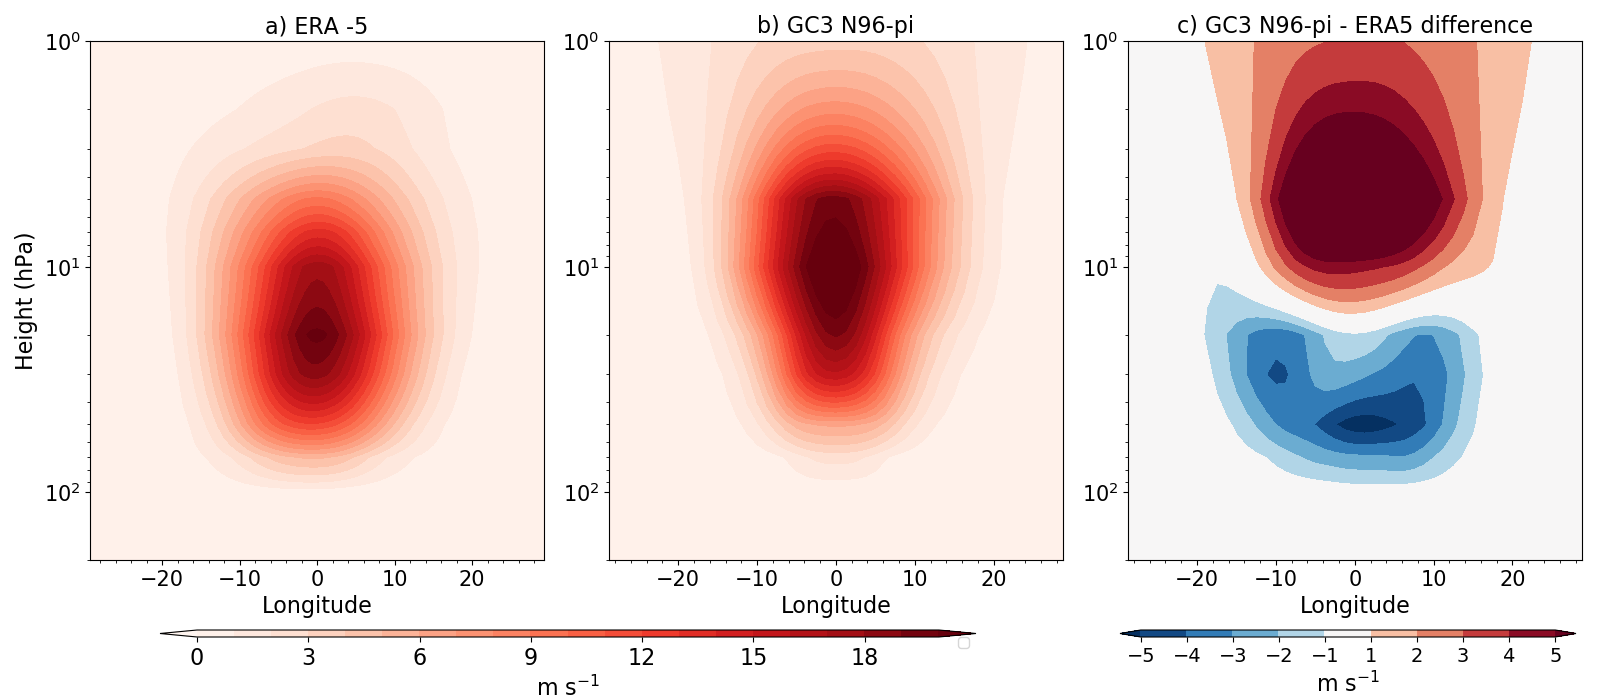
\includegraphics[width=\linewidth]{figures/qboamplitude.png}
\caption[QBO amplitude bias]{Latitude-pressure plot of the amplitude [m s$^{-1}$] of the QBO. Obtained from the zonal mean zonal wind fourier spectrum magnitude within the QBO periods, as in \cite{schenzinger2017}. }
\label{fig:qboamplitude}
\end{figure}

